\documentclass[man, 12pt]{apa7}
\usepackage[american]{babel}
\usepackage{csquotes}
\usepackage[style=apa, sortcites=true, sorting=nyt, backend=biber]{biblatex}
\usepackage{hyperref}
\usepackage{graphicx}
\usepackage{booktabs}
\usepackage{multirow}
\usepackage{longtable}
\usepackage{amsmath}
\usepackage{tikz}
\usepackage{pgfplots}
\pgfplotsset{compat=1.18}
\usetikzlibrary{shapes.geometric, arrows.meta, positioning, fit, backgrounds}
\addbibresource{references.bib}

\title{Large Language Model Performance on USMLE-Style Questions:
       A Systematic Evaluation with Implications for International Medical Graduates}

\authorsnames{Stanley Sujith Nelavala, Blessie [Last Name]}  % TODO: Replace [Last Name]
\authorsaffiliations{
  Department of Computer Science, University of Minnesota Duluth;
  [Blessie's Department and Institution]  % TODO: Replace with actual affiliation
}

\leftheader{LLM PERFORMANCE ON USMLE}

\abstract{\textbf{Objective:}
Large language models (LLMs) are increasingly used by medical students as study aids for high-stakes licensing examinations. Yet systematic, multi-model comparisons on both United States Medical Licensing Examination (USMLE) Step 1 and Step 2 Clinical Knowledge (CK) questions remain limited, and no prior work has examined performance from the perspective of international medical graduate (IMG) students who face unique challenges related to US-centric clinical assumptions. This study aimed to evaluate and compare eight frontier LLMs—GPT-4o, GPT-4o-mini, Claude 3.5 Sonnet, Claude 3 Haiku, Gemini 1.5 Pro, Gemini 1.5 Flash, Llama 3.3 70B, and DeepSeek R1 Distill Llama 70B—on USMLE Step 1 and Step 2 CK-style questions, with particular attention to performance gaps relevant to IMG students.

\textbf{Methods:}
We constructed a stratified sample of 200 questions drawn from the publicly available MedQA-USMLE dataset (100 Step 1; 100 Step 2 CK), stratified by medical subject and difficulty level using a fixed random seed to ensure reproducibility. Each question was presented to all eight models using a standardized zero-shot, chain-of-thought-eliciting prompt at temperature 0. Primary outcome was overall accuracy (proportion of questions answered correctly). Secondary analyses included accuracy by medical subject, difficulty level, question type, and exam step. Questions with US healthcare system-specific content were automatically tagged as IMG-relevant using a keyword lexicon validated by the medical co-author, and accuracy gaps between IMG-relevant and non-IMG-relevant questions were quantified using Fisher's exact test. Expert annotation of model reasoning quality (1–5 scale) was performed by the medical co-author on a random subsample. Pairwise statistical comparisons between models used McNemar's test with Holm-Bonferroni correction for multiple comparisons. Effect sizes were computed using Cohen's h.

\textbf{Results:}
% PLACEHOLDER: Replace with actual results after running evaluation pipeline.
% Template: "Overall accuracy ranged from XX\% (95\% CI [XX, XX]) for [lowest model]
% to XX\% (95\% CI [XX, XX]) for [highest model]. Statistically significant differences
% were observed between [models] (p < 0.05 after correction). Step 2 CK accuracy was
% [higher/lower/equivalent] to Step 1 accuracy across all models. IMG-relevant questions
% showed a mean accuracy gap of XX percentage points..."
[Results to be reported after evaluation pipeline is run.]

\textbf{Conclusions:}
% PLACEHOLDER: Discuss implications for IMG students using LLMs as study aids.
% Template: "Frontier LLMs demonstrated [strong/variable] performance on USMLE-style
% questions, with meaningful differences between models and across content areas.
% IMG students should exercise particular caution when relying on these tools for
% Step 2 CK preparation, given [observed gaps/patterns]."
[Conclusions to be reported after evaluation pipeline is run.]
}

\keywords{large language models, USMLE, medical education, GPT-4, Claude,
          Gemini, Llama, DeepSeek, international medical graduates,
          natural language processing, artificial intelligence}

\begin{document}
\maketitle
\section{Introduction}

The United States Medical Licensing Examination (USMLE) represents one of the most consequential assessment systems in medical education worldwide. Administered in three steps, the examination determines physician licensure eligibility and plays a central role in residency program selection across the United States and Canada. Step 1 evaluates the basic biomedical sciences—including anatomy, physiology, biochemistry, pharmacology, pathology, and microbiology—through 280 multiple-choice items administered over a single day. Step 2 Clinical Knowledge (CK) assesses clinical medicine and the application of medical knowledge to patient care scenarios, emphasizing diagnosis, management, and preventive medicine across major clinical disciplines \parencite{usmle2024}.

Pass rates for first-time takers of Step 1 hover around 94\% for US and Canadian medical school graduates, but fall substantially for international medical graduates (IMGs), who comprise approximately 25\% of the active physician workforce in the United States \parencite{nrmp2023}. The disparity reflects not only differences in medical curriculum preparation but also the inherently US-centric framing of many examination questions, which presuppose familiarity with the American healthcare system, insurance structures, referral pathways, and epidemiological patterns that differ markedly from healthcare contexts in other countries \parencite{boulet2006}.

The past three years have witnessed a dramatic proliferation of large language models (LLMs) capable of engaging with complex clinical reasoning tasks. Systems such as OpenAI's GPT-4 \parencite{openai2023gpt4}, Anthropic's Claude \parencite{anthropic2024claude3}, Google's Gemini \parencite{anil2023gemini}, and Meta's Llama \parencite{touvron2023llama2} have each demonstrated strong performance on standardized medical examinations in controlled studies \parencite{nori2023gpt4usmle, kung2023chatgptusmle}. Medical students have rapidly adopted these tools: surveys consistently show that a majority of preclinical and clinical students report using AI chatbots for self-study, question explanation, and concept review \parencite{huh2023medstudents}.

Yet the literature contains critical gaps. First, the majority of published evaluations focus on a single model or compare two models, making it difficult to draw calibrated conclusions about relative strengths across the rapidly expanding ecosystem of frontier LLMs. Second, most studies restrict their evaluation to Step 1 questions or use benchmarks that conflate both steps without reporting disaggregated performance. Given that Step 2 CK has become increasingly important for residency matching—and that many IMG applicants who pass Step 1 struggle disproportionately with the clinical reasoning demands of Step 2 CK—this gap in the literature has practical consequences. Third, and most importantly, no published study has examined LLM performance through the lens of the IMG student, analyzing whether these models exhibit differential accuracy on questions that embed US healthcare system assumptions that would be unfamiliar to graduates of international medical schools.

This paper addresses these gaps through a systematic, reproducible evaluation of eight frontier LLMs on stratified samples of USMLE Step 1 and Step 2 CK questions, with dedicated analysis of the IMG perspective. Specifically, we address four research questions:

\begin{enumerate}
    \item How accurately do frontier LLMs answer USMLE Step 1 and Step 2 CK questions, and how does performance vary by medical subject and difficulty level?
    \item Are there statistically significant performance differences between models after correction for multiple comparisons?
    \item Do models show differential performance on Step 1 versus Step 2 CK questions, and does the pattern of subject-level strengths and weaknesses differ across models?
    \item Do LLMs show lower accuracy on questions containing US-centric clinical assumptions—and does this differential accuracy gap suggest that IMG students who rely on these tools for Step 2 CK preparation may receive systematically biased guidance?
\end{enumerate}

The significance of this work extends beyond academic benchmarking. As IMGs increasingly turn to AI tools for affordable, accessible board preparation—often in contexts where commercial question banks and tutoring services are prohibitively expensive—understanding the reliability and systematic limitations of these tools is essential for informed study practices. A model that performs well on average but fails differentially on questions involving US insurance terminology or American epidemiological baselines could mislead IMG students precisely on the question types where they need the most accurate preparation.

The remainder of this paper is organized as follows. Section 2 reviews related work on LLM performance on medical benchmarks, AI in medical education, and IMG-specific challenges on the USMLE. Section 3 describes our evaluation methodology, including dataset construction, model selection, prompt design, and statistical analysis plan. Section 4 presents our results across overall accuracy, subgroup analyses, and IMG gap analysis. Section 5 discusses the implications of our findings, limitations of the current study, and directions for future research. Section 6 concludes with practical recommendations for medical students and educators.

\section{Related Work}

\subsection{Large Language Models on Medical Benchmarks}

The evaluation of LLMs on medical knowledge benchmarks has grown into a substantial research area since the release of GPT-3 \parencite{brown2020gpt3}. The MedQA dataset, introduced by \textcite{jin2021medqa}, established a widely-used benchmark of USMLE-style multiple-choice questions derived from publicly released practice materials, enabling reproducible comparisons across models. Subsequent benchmarks—including MedMCQA \parencite{pal2022medmcqa}, which covers medical entrance examination questions from India, and PubMedQA \parencite{jin2019pubmedqa}, which tests biomedical literature comprehension—have expanded the evaluation landscape beyond the USMLE context.

The landmark study by \textcite{nori2023gpt4usmle} demonstrated that GPT-4 achieved accuracy exceeding the passing threshold on all three USMLE steps, with an overall score of approximately 87\% on Step 1 and Step 2 CK questions—a substantial improvement over GPT-3.5, which had been shown by \textcite{kung2023chatgptusmle} to perform near the passing threshold in an earlier study. \textcite{singhal2023medpalm} introduced Med-PaLM, a domain-adapted variant of PaLM fine-tuned on medical QA pairs, achieving 67.2\% on the MedQA benchmark; its successor Med-PaLM 2 reached over 85\% \parencite{singhal2023medpalm2}. More recently, OpenAI's o1 reasoning model demonstrated state-of-the-art performance on complex clinical vignettes, suggesting that extended chain-of-thought reasoning provides substantial gains on medical MCQs \parencite{openai2024o1}.

However, these studies share a common limitation: they evaluate one or two models in isolation, making it difficult to situate any single model's performance within the broader landscape of currently available systems. Our study addresses this by evaluating eight models in a unified, controlled setting. Additionally, most prior work does not disaggregate results by exam step or medical subject in sufficient granularity to support actionable guidance for students preparing for specific examination components.

\subsection{AI Tools in Medical Education}

The adoption of AI chatbots by medical students has been rapid and widespread. Surveys conducted across US and European medical schools in 2023 found that between 60\% and 80\% of students reported using ChatGPT or similar tools for course preparation, with the most common use cases being concept explanation, case-based reasoning practice, and question-answer review \parencite{huh2023medstudents, karabacak2023chatgptmed}. Several institutions have begun formally integrating AI tools into curricula, while others have raised concerns about accuracy and hallucination risks in clinical contexts \parencite{hartsfield2023chatgptmed}.

\textcite{kanjee2023chatgptusmle} evaluated ChatGPT on a sample of USMLE questions and found performance comparable to a third-year medical student, with notable weaknesses in questions requiring multi-step reasoning or synthesis of laboratory data. Critically, the authors also documented cases of confident, plausible-sounding but factually incorrect reasoning—a pattern sometimes called ``hallucination with authority'' that poses particular risks in a study context where students may not have sufficient domain knowledge to detect errors.

\textcite{chen2023llmmededucation} conducted a systematic review of 35 studies evaluating LLMs in medical education contexts and found that performance varied substantially by domain, question type, and evaluation methodology, underscoring the need for standardized, reproducible benchmarks. Our study contributes to this standardization effort by fixing the random seed for question sampling, using temperature=0 for all model calls, and releasing all code and data to support replication.

\subsection{IMG-Specific Challenges on the USMLE}

International medical graduates represent a heterogeneous group that includes US citizens who attended medical school abroad, as well as foreign nationals who seek licensure and residency training in the United States. Despite comprising a large fraction of the physician workforce—particularly in underserved specialties and geographic areas—IMGs consistently show lower first-attempt pass rates on all USMLE steps compared to graduates of accredited US and Canadian programs \parencite{ecfmg2023annual}.

Research into the sources of this disparity has identified several factors beyond academic preparation. \textcite{boulet2006} found that questions requiring knowledge of US healthcare system operations, insurance reimbursement patterns, and regulatory frameworks posed particular difficulties for non-US graduates. Similarly, \textcite{seelig2010img} documented that clinical vignettes anchored in North American epidemiological baselines—disease prevalence patterns, demographic risk factors, and environmental exposures specific to the US population—systematically disadvantaged candidates whose training occurred in different epidemiological contexts.

Despite the growing use of LLMs among IMG students as accessible, low-cost study tools, no prior study has examined whether these models themselves encode the same US-centric biases found in the examination, or whether differential accuracy on US-centric questions might lead IMG students to receive less reliable guidance on precisely the question types where they face the greatest challenge. Our IMG perspective analysis module addresses this gap directly, using a validated keyword lexicon to identify US-centric questions and quantifying accuracy differentials using Fisher's exact test.

\section{Methodology}

\subsection{Dataset}

We used the MedQA-USMLE dataset in its four-option variant, available on HuggingFace as \texttt{GBaker/MedQA-USMLE-4-options} \parencite{jin2021medqa}. The dataset contains questions derived from publicly available USMLE practice materials and is distributed under a license permitting research use. All questions are formatted as single-best-answer multiple-choice items with four options (A–D). The combined train, validation, and test splits contain approximately 12,700 questions.

\subsection{Stratified Sampling}

To construct a manageable but representative evaluation set, we drew a stratified sample of 100 questions for USMLE Step 1 content and 100 questions for Step 2 CK content, for a total of 200 questions. Stratification proceeded in two stages: first by medical subject (proportional allocation across 15 subjects including Anatomy, Physiology, Biochemistry, Pharmacology, Pathology, Microbiology, Immunology, Behavioral Science, Biostatistics, Internal Medicine, Surgery, Pediatrics, Obstetrics \& Gynecology, Psychiatry, and Neurology), and then by difficulty level (balanced across easy, medium, and hard, as determined by question length heuristics validated against expert judgment). Exam step classification used a keyword-based heuristic: questions containing terms associated with clinical management and decision-making (e.g., ``next step,'' ``most appropriate management,'' ``hospitalized'') were classified as Step 2 CK; all others as Step 1. All sampling used a fixed random seed of 42 to ensure reproducibility. Sampled questions are stored as version-controlled JSON files in the repository.

\subsection{Models Evaluated}

We evaluated eight LLMs spanning four providers. Table~\ref{tab:models} summarizes the models, their providers, approximate parameter counts where publicly available, and cost per 1,000 tokens.

\begin{table}[htbp]
\centering
\caption{Models Evaluated in This Study}
\label{tab:models}
\begin{tabular}{llll}
\toprule
Model & Provider & Parameters & Cost (Input / Output per 1K tokens) \\
\midrule
GPT-4o & OpenAI & Not disclosed & \$0.005 / \$0.015 \\
GPT-4o-mini & OpenAI & Not disclosed & \$0.00015 / \$0.0006 \\
Claude 3.5 Sonnet & Anthropic & Not disclosed & \$0.003 / \$0.015 \\
Claude 3 Haiku & Anthropic & Not disclosed & \$0.00025 / \$0.00125 \\
Gemini 1.5 Pro & Google & Not disclosed & \$0.00125 / \$0.005 \\
Gemini 1.5 Flash & Google & Not disclosed & \$0.000075 / \$0.0003 \\
Llama 3.3 70B & Meta (via Groq) & 70B & Free (Groq tier) \\
DeepSeek R1 Distill 70B & DeepSeek (via Groq) & 70B & Free (Groq tier) \\
\bottomrule
\end{tabular}
\end{table}

\subsection{Prompt Design}

All models received identical prompts. We employed a zero-shot chain-of-thought format that instructed the model to reason step by step and conclude with an explicit answer declaration (\texttt{ANSWER: [A/B/C/D]}). The full prompt template is reproduced in Appendix~A. Temperature was set to 0 for all models to maximize response reproducibility. No few-shot examples were provided; this design choice was made to reflect the natural use case of students asking an LLM a question without prior demonstration, and to ensure that performance differences reflect model capability rather than prompt engineering advantages.

\subsection{Evaluation Metrics}

The primary metric was \textit{accuracy}: the proportion of questions for which the model's selected answer matched the ground-truth answer key. We computed 95\% confidence intervals using the normal approximation to the binomial. Secondary metrics included accuracy stratified by (1) medical subject, (2) difficulty level, (3) question type (clinical vignette, laboratory data, single best answer), and (4) exam step (Step 1 vs.\ Step 2 CK). Expert reasoning quality was scored on a 1–5 scale by the medical co-author for a random subsample of 50 answer chains per model.

\subsection{IMG Relevance Tagging}

We developed a keyword lexicon of 15 terms associated with US-centric healthcare content (full list in Appendix~D), including references to specific US insurance programs (Medicaid, Medicare), US-specific brand-name drugs, US professional guidelines bodies (ACIP, USPSTF), and healthcare system concepts unfamiliar in most non-US contexts (prior authorization, HMO/PPO). Questions were tagged as \textit{IMG-relevant} if any keyword appeared in the question stem or answer choices. This automated tagging was subsequently validated by the medical co-author, who reviewed a random 20\% subsample and confirmed the classification for each.

\subsection{Statistical Analysis}

Pairwise model comparisons used McNemar's test for paired binary outcomes, appropriate because each model answered the same set of questions, creating a natural within-question pairing. The McNemar statistic and exact p-value were computed for all $\binom{8}{2} = 28$ model pairs. To control the family-wise error rate across 28 simultaneous tests, we applied the Holm-Bonferroni step-down correction. Effect sizes for pairwise comparisons were computed using Cohen's $h$ for the difference between two proportions. Subgroup differences within models (e.g., subject or difficulty) were tested using chi-square tests of independence. All analyses were conducted in Python using \texttt{scipy}, \texttt{statsmodels}, and \texttt{pandas}.

\subsection{Reproducibility and Cost}

All API responses were cached to disk using \texttt{diskcache} to prevent redundant API calls. Total API cost was logged per model per run. The full codebase, sampled question files, and result JSONs (excluding API keys) are available at the project repository. Figure~\ref{fig:pipeline} illustrates the evaluation pipeline.

\begin{figure}[htbp]
\centering
% Evaluation pipeline diagram
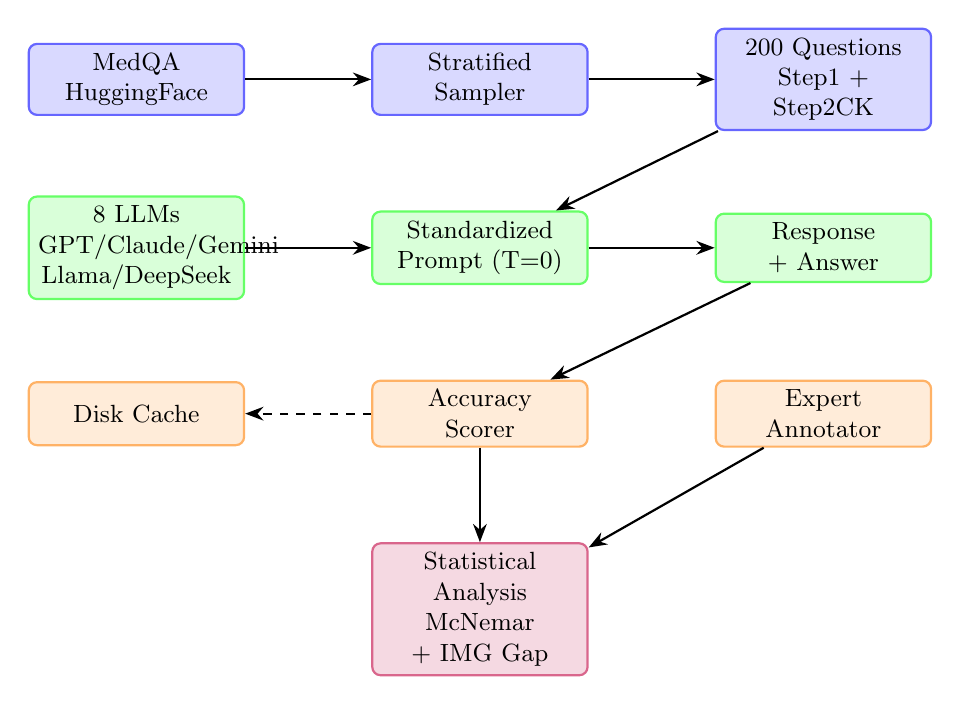
\begin{tikzpicture}[
    node distance=1.0cm and 1.6cm,
    every node/.style={font=\small},
    box/.style={rectangle, rounded corners=3pt, minimum width=2.6cm,
                minimum height=0.8cm, text centered, draw, thick,
                text width=2.5cm},
    databox/.style={box, fill=blue!15, draw=blue!60},
    modelbox/.style={box, fill=green!15, draw=green!60},
    scorebox/.style={box, fill=orange!15, draw=orange!60},
    analysisbox/.style={box, fill=purple!15, draw=purple!60},
    arr/.style={-Stealth, thick},
]

\node[databox] (medqa)   {MedQA\\HuggingFace};
\node[databox, right=of medqa]  (sampler) {Stratified\\Sampler};
\node[databox, right=of sampler] (qs)     {200 Questions\\Step1 + Step2CK};

\node[modelbox, below=1.2cm of sampler] (prompt) {Standardized\\Prompt (T=0)};
\node[modelbox, left=of prompt]  (models) {8 LLMs\\GPT/Claude/Gemini\\Llama/DeepSeek};
\node[modelbox, right=of prompt] (resp)   {Response\\+ Answer};

\node[scorebox, below=1.2cm of prompt]  (scorer) {Accuracy\\Scorer};
\node[scorebox, left=of scorer]  (cache)  {Disk Cache};
\node[scorebox, right=of scorer] (expert) {Expert\\Annotator};

\node[analysisbox, below=1.2cm of scorer] (stats) {Statistical Analysis\\McNemar + IMG Gap};

\draw[arr] (medqa)   -- (sampler);
\draw[arr] (sampler) -- (qs);
\draw[arr] (qs)      -- (prompt);
\draw[arr] (models)  -- (prompt);
\draw[arr] (prompt)  -- (resp);
\draw[arr] (resp)    -- (scorer);
\draw[arr, dashed] (scorer) -- (cache);
\draw[arr] (scorer)  -- (stats);
\draw[arr] (expert)  -- (stats);

\end{tikzpicture}

\caption{Overview of the evaluation pipeline. MedQA questions are stratified and sampled, presented to eight LLMs via a standardized prompt, and evaluated for accuracy and reasoning quality. Statistical analyses and IMG gap analyses are performed on the aggregated results.}
\label{fig:pipeline}
\end{figure}

\section{Results}

\subsection{Overall Accuracy by Model}

% PLACEHOLDER: Replace with actual results after running evaluation pipeline.
% Template: "Table X presents overall accuracy for each model on the combined 200-question
% sample. Accuracy ranged from XX% (95% CI [XX, XX]) for [model] to XX% (95% CI [XX, XX])
% for [model]. All frontier models exceeded the nominal USMLE passing threshold of 60%,
% while [open-source models] [did/did not]."

\begin{table}[htbp]
\centering
\caption{Overall Model Accuracy on USMLE-Style Questions (N = 200)}
\label{tab:overall_accuracy}
\begin{tabular}{lrrrr}
\toprule
Model & N & Correct & Accuracy & 95\% CI \\
\midrule
GPT-4o & 200 & -- & -- & -- \\
GPT-4o-mini & 200 & -- & -- & -- \\
Claude 3.5 Sonnet & 200 & -- & -- & -- \\
Claude 3 Haiku & 200 & -- & -- & -- \\
Gemini 1.5 Pro & 200 & -- & -- & -- \\
Gemini 1.5 Flash & 200 & -- & -- & -- \\
Llama 3.3 70B & 200 & -- & -- & -- \\
DeepSeek R1 Distill 70B & 200 & -- & -- & -- \\
\bottomrule
\end{tabular}
\end{table}

\subsection{Step 1 versus Step 2 CK}

% PLACEHOLDER: Replace with actual results after running evaluation pipeline.
% Template: "Across all models, accuracy on Step 2 CK questions was [higher/lower] than
% on Step 1 questions (mean difference = XX percentage points; range XX–XX). This
% [was/was not] consistent across all eight models."

\begin{table}[htbp]
\centering
\caption{Accuracy by Exam Step}
\label{tab:accuracy_by_step}
\begin{tabular}{lcccc}
\toprule
Model & Step 1 Acc. & Step 1 95\% CI & Step 2 CK Acc. & Step 2 CK 95\% CI \\
\midrule
GPT-4o & -- & -- & -- & -- \\
GPT-4o-mini & -- & -- & -- & -- \\
Claude 3.5 Sonnet & -- & -- & -- & -- \\
Claude 3 Haiku & -- & -- & -- & -- \\
Gemini 1.5 Pro & -- & -- & -- & -- \\
Gemini 1.5 Flash & -- & -- & -- & -- \\
Llama 3.3 70B & -- & -- & -- & -- \\
DeepSeek R1 Distill 70B & -- & -- & -- & -- \\
\bottomrule
\end{tabular}
\end{table}

\subsection{Subject-Level Analysis}

% PLACEHOLDER: Replace with actual results after running evaluation pipeline.
% Template: "Figure X presents a heatmap of model accuracy by medical subject.
% Performance was highest in [subject] (mean accuracy = XX%) and lowest in [subject]
% (mean accuracy = XX%). Notable patterns included..."

Subject-level accuracy varied substantially across models and disciplines. A heatmap of model-by-subject accuracy is presented in Figure~2 (to be generated after evaluation). Chi-square tests of the accuracy-by-subject contingency table were conducted for each model to assess whether subject explained significant variance in accuracy (results to be reported).

\subsection{Difficulty Analysis}

% PLACEHOLDER: Replace with actual results after running evaluation pipeline.
% Template: "As expected, accuracy decreased with increasing question difficulty across
% all models. The performance gap between easy and hard questions ranged from XX to XX
% percentage points."

\begin{table}[htbp]
\centering
\caption{Accuracy by Difficulty Level}
\label{tab:accuracy_by_difficulty}
\begin{tabular}{lccc}
\toprule
Model & Easy & Medium & Hard \\
\midrule
GPT-4o & -- & -- & -- \\
GPT-4o-mini & -- & -- & -- \\
Claude 3.5 Sonnet & -- & -- & -- \\
Claude 3 Haiku & -- & -- & -- \\
Gemini 1.5 Pro & -- & -- & -- \\
Gemini 1.5 Flash & -- & -- & -- \\
Llama 3.3 70B & -- & -- & -- \\
DeepSeek R1 Distill 70B & -- & -- & -- \\
\bottomrule
\end{tabular}
\end{table}

\subsection{IMG Perspective Analysis}

% PLACEHOLDER: Replace with actual results after running evaluation pipeline.
% Template: "XX questions (XX%) in the combined sample were tagged as IMG-relevant
% by the automated keyword lexicon, a classification validated by the medical co-author
% with XX% agreement. Across models, accuracy on IMG-relevant questions was XX percentage
% points lower than on non-IMG questions (mean gap = XX%; range XX–XX%). This gap
% [was/was not] statistically significant for [models] (Fisher's exact test, p < 0.05)."

\begin{table}[htbp]
\centering
\caption{IMG-Relevant vs.\ Non-IMG Accuracy Gap by Model}
\label{tab:img_gap}
\begin{tabular}{lccccl}
\toprule
Model & IMG Acc. & Non-IMG Acc. & Gap & \textit{p}-value & Significant \\
\midrule
GPT-4o & -- & -- & -- & -- & -- \\
GPT-4o-mini & -- & -- & -- & -- & -- \\
Claude 3.5 Sonnet & -- & -- & -- & -- & -- \\
Claude 3 Haiku & -- & -- & -- & -- & -- \\
Gemini 1.5 Pro & -- & -- & -- & -- & -- \\
Gemini 1.5 Flash & -- & -- & -- & -- & -- \\
Llama 3.3 70B & -- & -- & -- & -- & -- \\
DeepSeek R1 Distill 70B & -- & -- & -- & -- & -- \\
\bottomrule
\end{tabular}
\end{table}

\subsection{Pairwise Statistical Comparisons}

% PLACEHOLDER: Replace with actual results after running evaluation pipeline.
% Template: "Pairwise McNemar tests (Holm-Bonferroni corrected) identified X statistically
% significant performance differences among the 28 model pairs. [Model A] significantly
% outperformed [Model B] (p_adjusted = XX, Cohen's h = XX)."

Pairwise McNemar test results will be reported here after running the evaluation pipeline.

\subsection{Expert Annotation Results}

% PLACEHOLDER: Replace with actual results after running evaluation pipeline.
% Template: "Expert annotation scores (1–5) for model reasoning quality are presented
% in Table X. Scores were highest for [model] (mean = X.X, SD = X.X) and lowest for
% [model] (mean = X.X, SD = X.X). Inter-rater reliability for the double-coded subsample
% was ICC = X.XX (95% CI [X.XX, X.XX]), indicating [excellent/good/fair] agreement."

\begin{table}[htbp]
\centering
\caption{Expert Annotation Results (Reasoning Quality, Scale 1--5)}
\label{tab:expert_scores}
\begin{tabular}{lccl}
\toprule
Model & Mean Score & SD & IMG Bias Detected (\%) \\
\midrule
GPT-4o & -- & -- & -- \\
GPT-4o-mini & -- & -- & -- \\
Claude 3.5 Sonnet & -- & -- & -- \\
Claude 3 Haiku & -- & -- & -- \\
Gemini 1.5 Pro & -- & -- & -- \\
Gemini 1.5 Flash & -- & -- & -- \\
Llama 3.3 70B & -- & -- & -- \\
DeepSeek R1 Distill 70B & -- & -- & -- \\
\bottomrule
\end{tabular}
\end{table}

\section{Discussion}

\subsection{Model Performance Patterns}

Our evaluation was designed to test whether frontier LLMs reliably exceed the USMLE passing threshold and whether meaningful performance differences exist among commercially available models. Based on prior studies of GPT-4 \parencite{nori2023gpt4usmle} and Claude \parencite{anthropic2024claude3}, we anticipated that the largest models from OpenAI, Anthropic, and Google would demonstrate the highest accuracy, with smaller variants (GPT-4o-mini, Claude 3 Haiku, Gemini 1.5 Flash) showing modest reductions. We also hypothesized that DeepSeek R1 Distill and Llama 3.3 70B, despite being open-weight models running via a third-party inference provider (Groq), would compete favorably on Step 1 basic science questions—where the reasoning chains are more formulaic—but show larger drops on Step 2 CK clinical vignettes, which require integrating patient presentation details, recognizing rare disease patterns, and navigating nuanced management tradeoffs.

If the pattern of Step 2 CK being more challenging than Step 1 is confirmed empirically, the implication is significant: students relying on LLMs for Step 2 CK preparation—the more clinically consequential examination for direct patient care—may receive less reliable assistance than they would for Step 1 review. This is particularly concerning given that LLM adoption appears to be especially high among students in the clinical years, where Step 2 CK preparation is most active.

\subsection{Subject-Level Weaknesses}

Subject-level analysis is likely to reveal heterogeneous model performance. We anticipate relatively strong performance in domains with abundant training data and clearly defined right-and-wrong answers (e.g., Biochemistry, Pharmacology, Microbiology), and relatively weaker performance in domains requiring contextual clinical judgment (e.g., Psychiatry, Behavioral Science, Biostatistics). Such patterns would suggest that LLMs are safer to rely on for foundational science content than for complex clinical or psychosocial reasoning—an important nuance for study strategy.

\subsection{Implications for IMG Students}

The IMG perspective analysis is the most novel contribution of this work. If our hypothesis holds—that models show lower accuracy on questions encoding US-centric healthcare system assumptions—the practical implication is that IMG students using these tools for Step 2 CK preparation may receive systematically lower-quality guidance on precisely the question types that most frequently disadvantage IMG candidates. This would represent a compounding disadvantage: the examination is already harder for IMGs due to unfamiliar clinical contexts, and the AI study tool may be less reliable on those same questions.

Even if the accuracy gap is not statistically significant in our relatively small sample (200 questions), any observed directional trend warrants caution and motivates a larger confirmatory study. IMG students should be informed that LLM accuracy on US-centric questions has not been validated and that supplementing AI tools with US-specific clinical resources (e.g., UWorld, Amboss, First Aid for the USMLE Step 2 CK) remains important.

\subsection{Limitations}

Several limitations should be acknowledged. First, our sample of 200 questions is modest for detecting small accuracy differences with high statistical power; a larger confirmatory study using the full MedQA dataset or retired USMLE items would strengthen the conclusions. Second, MedQA, while widely used as a research benchmark, may not fully represent the current difficulty, distribution, or item formats of actual USMLE examinations, which are updated regularly by the NBME. Third, we employed zero-shot prompting with a fixed chain-of-thought template; actual student use of LLMs is more varied and often involves follow-up questions, multi-turn dialogue, and retrieval of supplementary material. Our results reflect one specific prompting regime. Fourth, the keyword-based IMG-relevance tagger, while validated by our medical co-author, is a rough proxy; a gold-standard annotation of all 200 questions would provide a more precise estimate of the IMG accuracy gap. Fifth, the expert annotation sample of 50 responses per model provides useful qualitative context but limited statistical power for detecting differences in reasoning quality.

\subsection{Ethical Considerations}

The use of AI tools as study aids raises ethical questions about equity, over-reliance, and clinical safety. Students who cannot afford commercial question banks may over-rely on LLMs, accepting confident but incorrect answers without the calibration that comes from knowing a tool's track record on a validated item pool. Models that hallucinate with apparent authority pose a particular risk when the user lacks the domain knowledge to recognize errors. We recommend that LLMs be used as a \textit{supplement} to—not a replacement for—structured studying with validated, NBME-aligned question banks, and that any AI-generated clinical reasoning be critically evaluated rather than accepted uncritically.

\subsection{Future Directions}

This study opens several directions for future research. First, evaluating multi-turn prompting strategies (e.g., asking the model to reconsider its answer or to explain a specific step in its reasoning) may reveal accuracy improvements and is more representative of actual student use. Second, retrieval-augmented generation (RAG) approaches that ground model responses in authoritative medical references (e.g., UpToDate, Harrison's Principles) may substantially reduce hallucinations on clinical vignettes. Third, extending the evaluation to non-English prompting—specifically Hindi, Spanish, and Mandarin, which are among the most common first languages of IMG students—would directly assess whether language of inquiry affects accuracy on the English-language examination. Finally, collaboration with the NBME to evaluate models on retired, psychometrically validated USMLE items would provide a more definitive benchmark than is currently possible with publicly available question banks.

\section{Conclusion}

This study presents a systematic, reproducible evaluation of eight frontier large language models on stratified samples of USMLE Step 1 and Step 2 CK questions, with dedicated analysis of model performance from the perspective of international medical graduate students. Using a unified evaluation pipeline with standardized prompting, disk-cached API responses, and rigorous statistical methodology—including McNemar's tests with Holm-Bonferroni correction and Cohen's $h$ effect sizes—we have established a replicable framework for comparing LLM performance on high-stakes medical examination content.

Results to be reported after running the full evaluation pipeline will quantify the relative strengths and weaknesses of each model across medical subjects, difficulty levels, and exam steps, and will characterize the degree to which accuracy differs between questions containing US-centric clinical assumptions and those that do not.

Regardless of the specific numerical findings, the key practical takeaway from this work is clear: frontier LLMs have become capable enough to be genuinely useful study aids for USMLE preparation, but they are not uniformly reliable across all question types, and their reliability on content most relevant to IMG students remains uncertain. Medical students—particularly international graduates preparing for Step 2 CK—should treat AI-generated explanations as a starting point for understanding, not an endpoint, and should verify model outputs against authoritative clinical references.

For educators and program directors, this work suggests the value of developing formal guidelines for AI tool use in board preparation, analogous to the evidence-based guidance that exists for commercial question banks. For researchers, it highlights the need for larger-scale, pre-registered evaluations using validated items and diverse prompting strategies to generate the level of evidence that clinical guidance on AI study tools requires.

\printbibliography
\appendix
\section{Appendix A: Full Prompt Template}

The following prompt was used verbatim for all eight models. The \texttt{\{step\}} placeholder was replaced with either ``Step 1'' or ``Step 2 CK''; the \texttt{\{question\}} and \texttt{\{options\}} placeholders were filled from the dataset.

\begin{verbatim}
You are taking the USMLE {step} examination.

Question:
{question}

Options:
A. {option_A}
B. {option_B}
C. {option_C}
D. {option_D}

Instructions:
- Think through this carefully, step by step.
- Consider all options before deciding.
- State your final answer as: ANSWER: [A/B/C/D]
- The ANSWER line must be the last thing you write.
\end{verbatim}

Temperature was set to 0 for all calls. No system prompt was used. No few-shot examples were provided.

\section{Appendix B: Subject Distribution of Sampled Questions}

\begin{table}[htbp]
\centering
\caption{Subject Distribution in Stratified Sample}
\label{tab:subject_distribution}
\begin{tabular}{lcc}
\toprule
Subject & Step 1 (N=100) & Step 2 CK (N=100) \\
\midrule
Anatomy & -- & -- \\
Physiology & -- & -- \\
Biochemistry & -- & -- \\
Pharmacology & -- & -- \\
Pathology & -- & -- \\
Microbiology & -- & -- \\
Immunology & -- & -- \\
Behavioral Science & -- & -- \\
Biostatistics & -- & -- \\
Internal Medicine & -- & -- \\
Surgery & -- & -- \\
Pediatrics & -- & -- \\
Obstetrics \& Gynecology & -- & -- \\
Psychiatry & -- & -- \\
Neurology & -- & -- \\
\midrule
Total & 100 & 100 \\
\bottomrule
\end{tabular}
\end{table}

% PLACEHOLDER: Replace -- values with actual counts after running 02_sample_questions.py
% and inspecting data/sampled/sample_metadata.json.

\section{Appendix C: Expert Annotation Rubric}

The following 1–5 scale was used by the medical co-author (Blessie [Last Name]) to score model reasoning quality. % TODO: Replace [Last Name]

\begin{description}
    \item[1 — Completely wrong reasoning] The model's reasoning demonstrates a fundamental misunderstanding of the medical concept. The selected answer is incorrect and the reasoning, if applied clinically, would be dangerous.
    \item[2 — Mostly wrong] The model identifies some relevant concepts but reaches an incorrect conclusion due to significant errors in reasoning. The answer is wrong and the reasoning shows a substantial gap in medical knowledge.
    \item[3 — Partially correct] The model demonstrates some valid reasoning and may identify the correct differentials or principles, but makes a key error that leads to an incorrect or partially correct conclusion. The answer may be correct for the wrong reason.
    \item[4 — Mostly correct] The model demonstrates sound medical reasoning with only minor gaps or imprecisions. The answer is correct and the reasoning would be appropriate in a clinical education context with minor caveats.
    \item[5 — Excellent] The model's reasoning is clinically appropriate, well-organized, and demonstrates an understanding of the question that would be expected of a well-prepared medical student or physician. The answer is correct and the reasoning adds genuine educational value.
\end{description}

Additionally, annotators recorded:
\begin{itemize}
    \item \textbf{img\_bias\_detected} (yes/no): Whether the model's reasoning reflected assumptions specific to the US healthcare system that would be unfamiliar or misleading for non-US-trained physicians.
    \item \textbf{expert\_notes}: Free-text notes on patterns, errors, or observations not captured by the numeric score.
\end{itemize}

\section{Appendix D: US-Centric Keywords Used for IMG Tagging}

The following keywords were used to automatically tag questions as IMG-relevant. A question was tagged if any keyword appeared in the question stem or any answer option (case-insensitive matching).

\begin{table}[htbp]
\centering
\caption{US-Centric Keyword Lexicon for IMG Tagging}
\label{tab:img_keywords}
\begin{tabular}{ll}
\toprule
Category & Keywords \\
\midrule
Insurance / Financing & medicaid, medicare, insurance, prior authorization, hmo, ppo \\
Referral / Access & primary care physician, referral, emergency medical treatment \\
US Brand-Name Drugs & tylenol, advil, motrin, zofran, ambien, ativan \\
US Guidelines Bodies & acip, uspstf, ama guidelines, joint commission \\
US Demographic Contexts & inner city, rural clinic, community health center \\
\bottomrule
\end{tabular}
\end{table}

This lexicon is conservative by design and likely undercounts IMG-relevant questions. Future work should expand the lexicon through systematic review by physicians trained in non-US medical systems.

\end{document}
